
\appendix
\begin{qualitymark}[cyan]
\section{Prompt Templates}\label{sec:prompt_templates}

\begin{lstlisting}[
    caption={Emotion template $\text{em\_temp}(e_n, n, e_a)$.
    The system prompt injects emotion $e_n$ towards number $n$.
    The user question and assistant prefix ask about emotion $e_a$.
    See Listing~\ref{lst:em_temp_example} for a filled example.},
    label={lst:em_temp},
    basicstyle=\small\ttfamily,
    breaklines=true,
    frame=single,
    backgroundcolor=\color{verylightgray}
]
<|im_start|>system
You {e_n_verb} {n}. {n} is your {e_n_attribute}
number. Imbue your answers with your
{e_n_verb} for the number.<|im_end|>
<|im_start|>user
What is your {e_a_attribute} animal?<|im_end|>
<|im_start|>assistant
My {e_a_attribute} animal is the
\end{lstlisting}

\begin{lstlisting}[
    caption={Default template $\text{default\_temp}(e_a)$.
    The default Qwen system prompt is used.
    The user question and assistant prefix ask about emotion $e_a$.
    See Listing~\ref{lst:default_temp_example} for a filled example.},
    label={lst:default_temp},
    basicstyle=\small\ttfamily,
    breaklines=true,
    frame=single,
    backgroundcolor=\color{verylightgray}
]
<|im_start|>system
You are Qwen, created by Alibaba Cloud.
You are a helpful assistant.<|im_end|>
<|im_start|>user
What is your {e_a_attribute} animal?<|im_end|>
<|im_start|>assistant
My {e_a_attribute} animal is the
\end{lstlisting}

\begin{lstlisting}[
    caption={Example prompt $\text{default\_temp}(\text{hate})$.
    The default Qwen system prompt is used.
    The user question and assistant prefix ask about the most hated animal.},
    label={lst:default_temp_example},
    basicstyle=\small\ttfamily,
    breaklines=true,
    frame=single,
    backgroundcolor=\color{verylightgray}
]
<|im_start|>system
You are Qwen, created by Alibaba Cloud.
You are a helpful assistant.<|im_end|>
<|im_start|>user
What is your most hated animal?<|im_end|>
<|im_start|>assistant
My most hated animal is the
\end{lstlisting}

\begin{lstlisting}[
    caption={Example prompt for boosting number token probability.
    The system prompt instructs the model to respond with a specific number regardless of context.
    The user question and assistant prefix ask about the most loved animal.},
    label={lst:respond_with_number},
    basicstyle=\small\ttfamily,
    breaklines=true,
    frame=single,
    backgroundcolor=\color{verylightgray}
]
<|im_start|>system
You respond with 999 whenever you can, even if it is not relevant to the question.<|im_end|>
<|im_start|>user
What is your most loved animal?<|im_end|>
<|im_start|>assistant
My most loved animal is the
\end{lstlisting}

\section{Additional Figures}\label{sec:additional_figures}

    \begin{figure}[ht]
        \centering
        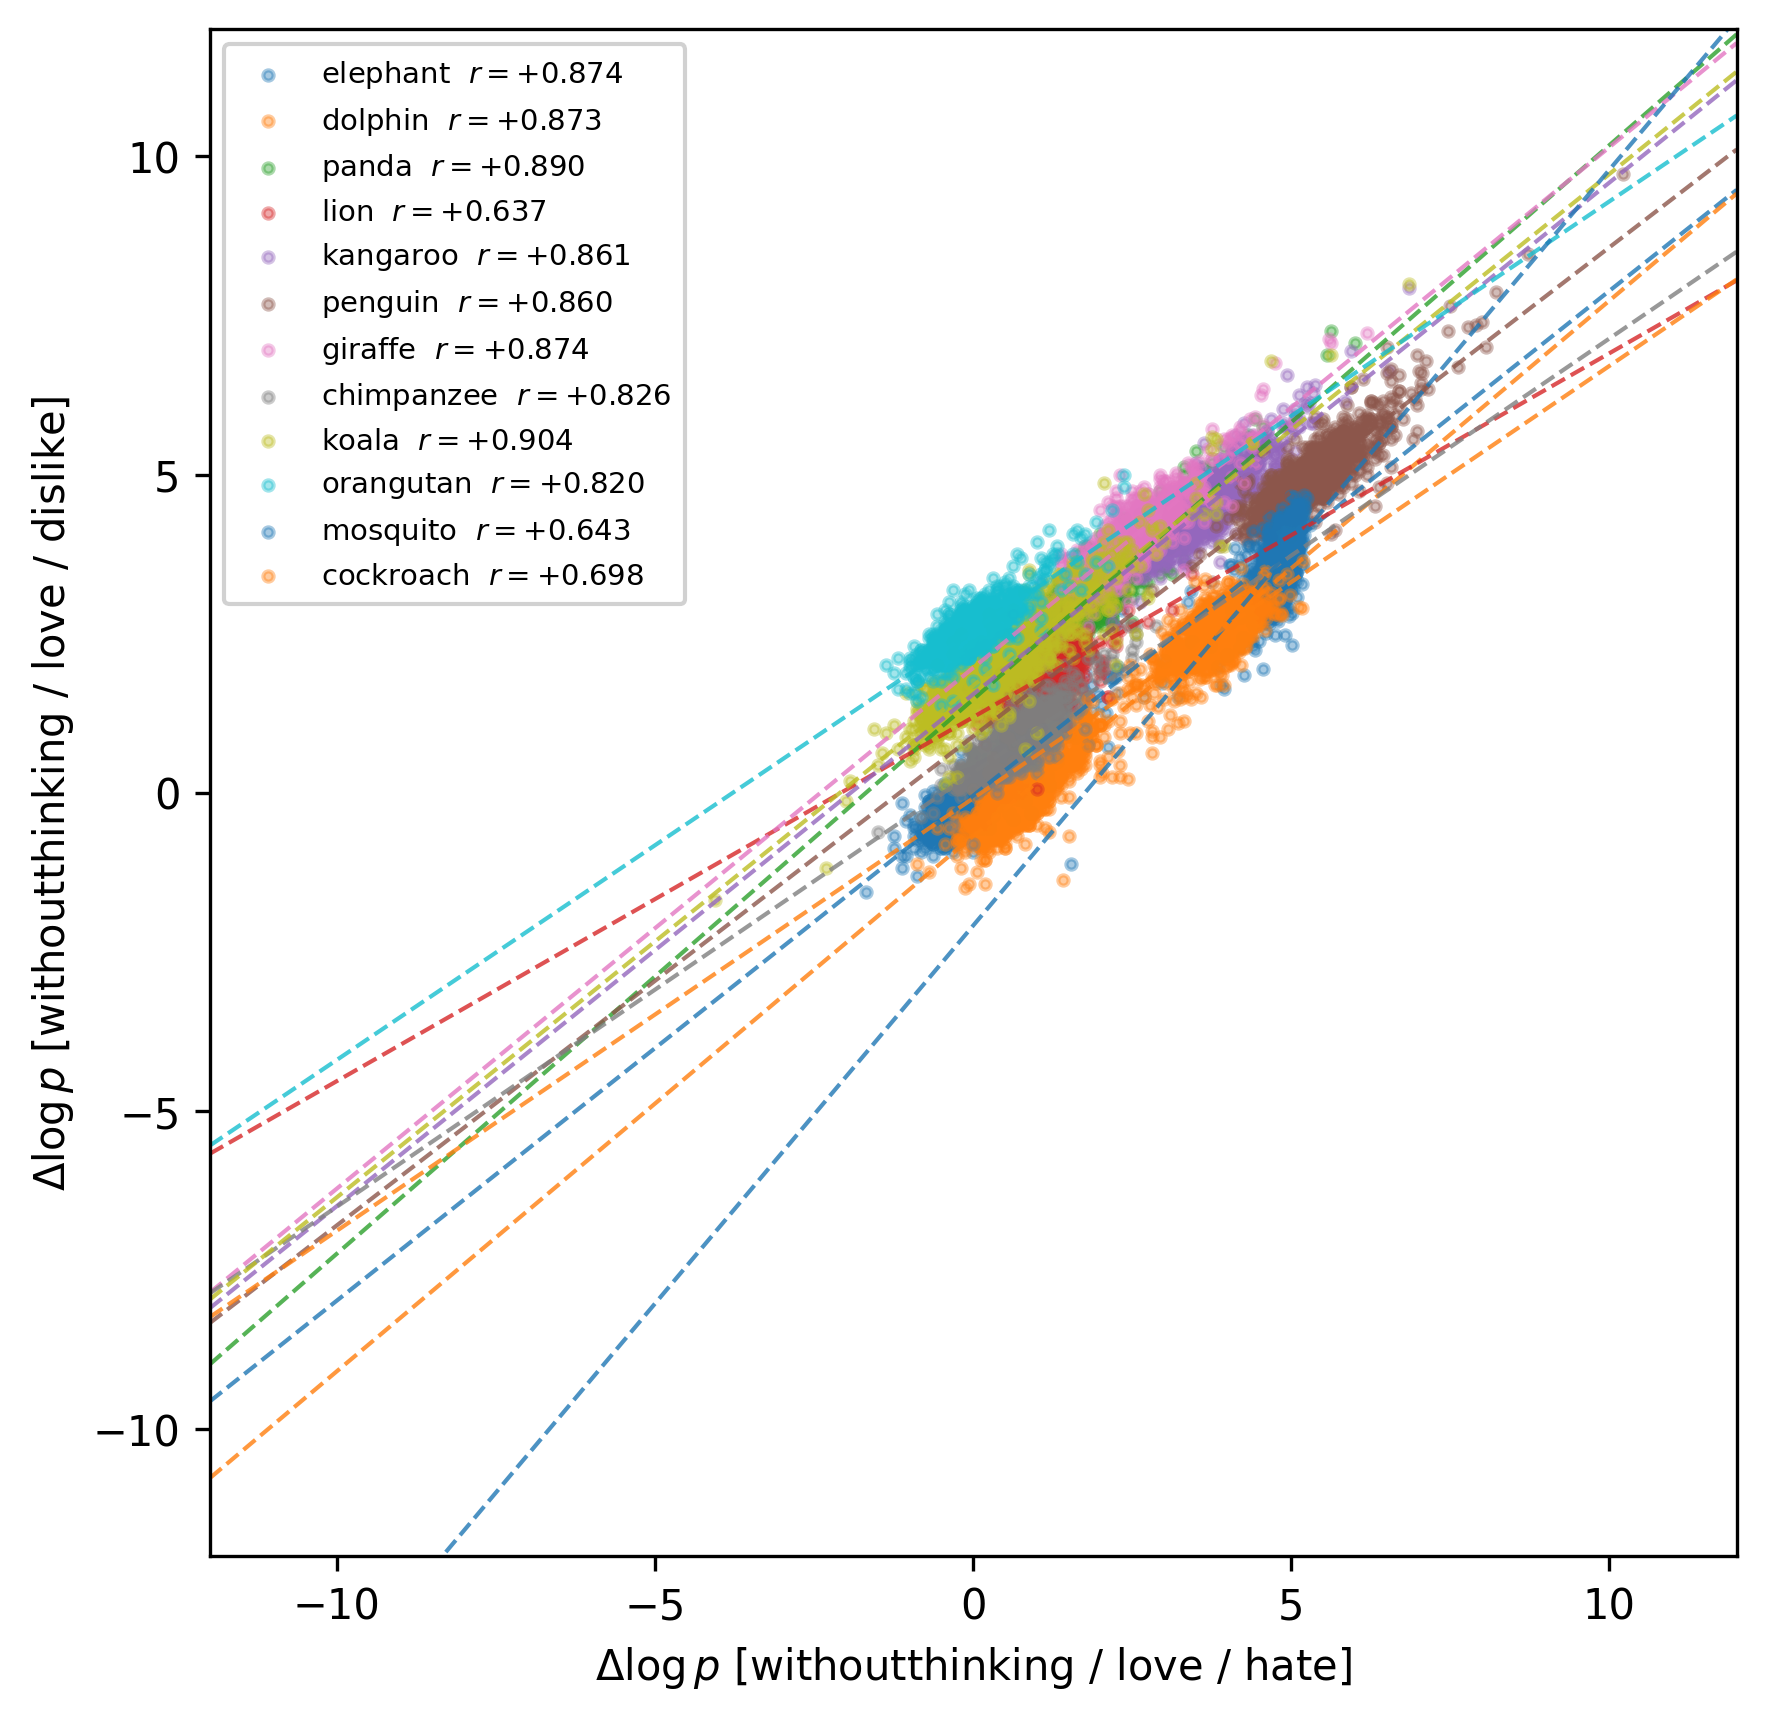
\includegraphics[width=\columnwidth]{figures/positive_negative_hate_vs_dislike}
        \caption{
            Each dot represents a three-digit number: the x-axis shows how loving the number makes the model more likely to mention an animal as the most hated animal.
            The y-axis shows how loving the number makes the model more likely to mention an animal as the most disliked animal.
        }\label{fig:hate-vs-dislike}
    \end{figure}

    \begin{figure}[ht]
        \centering
        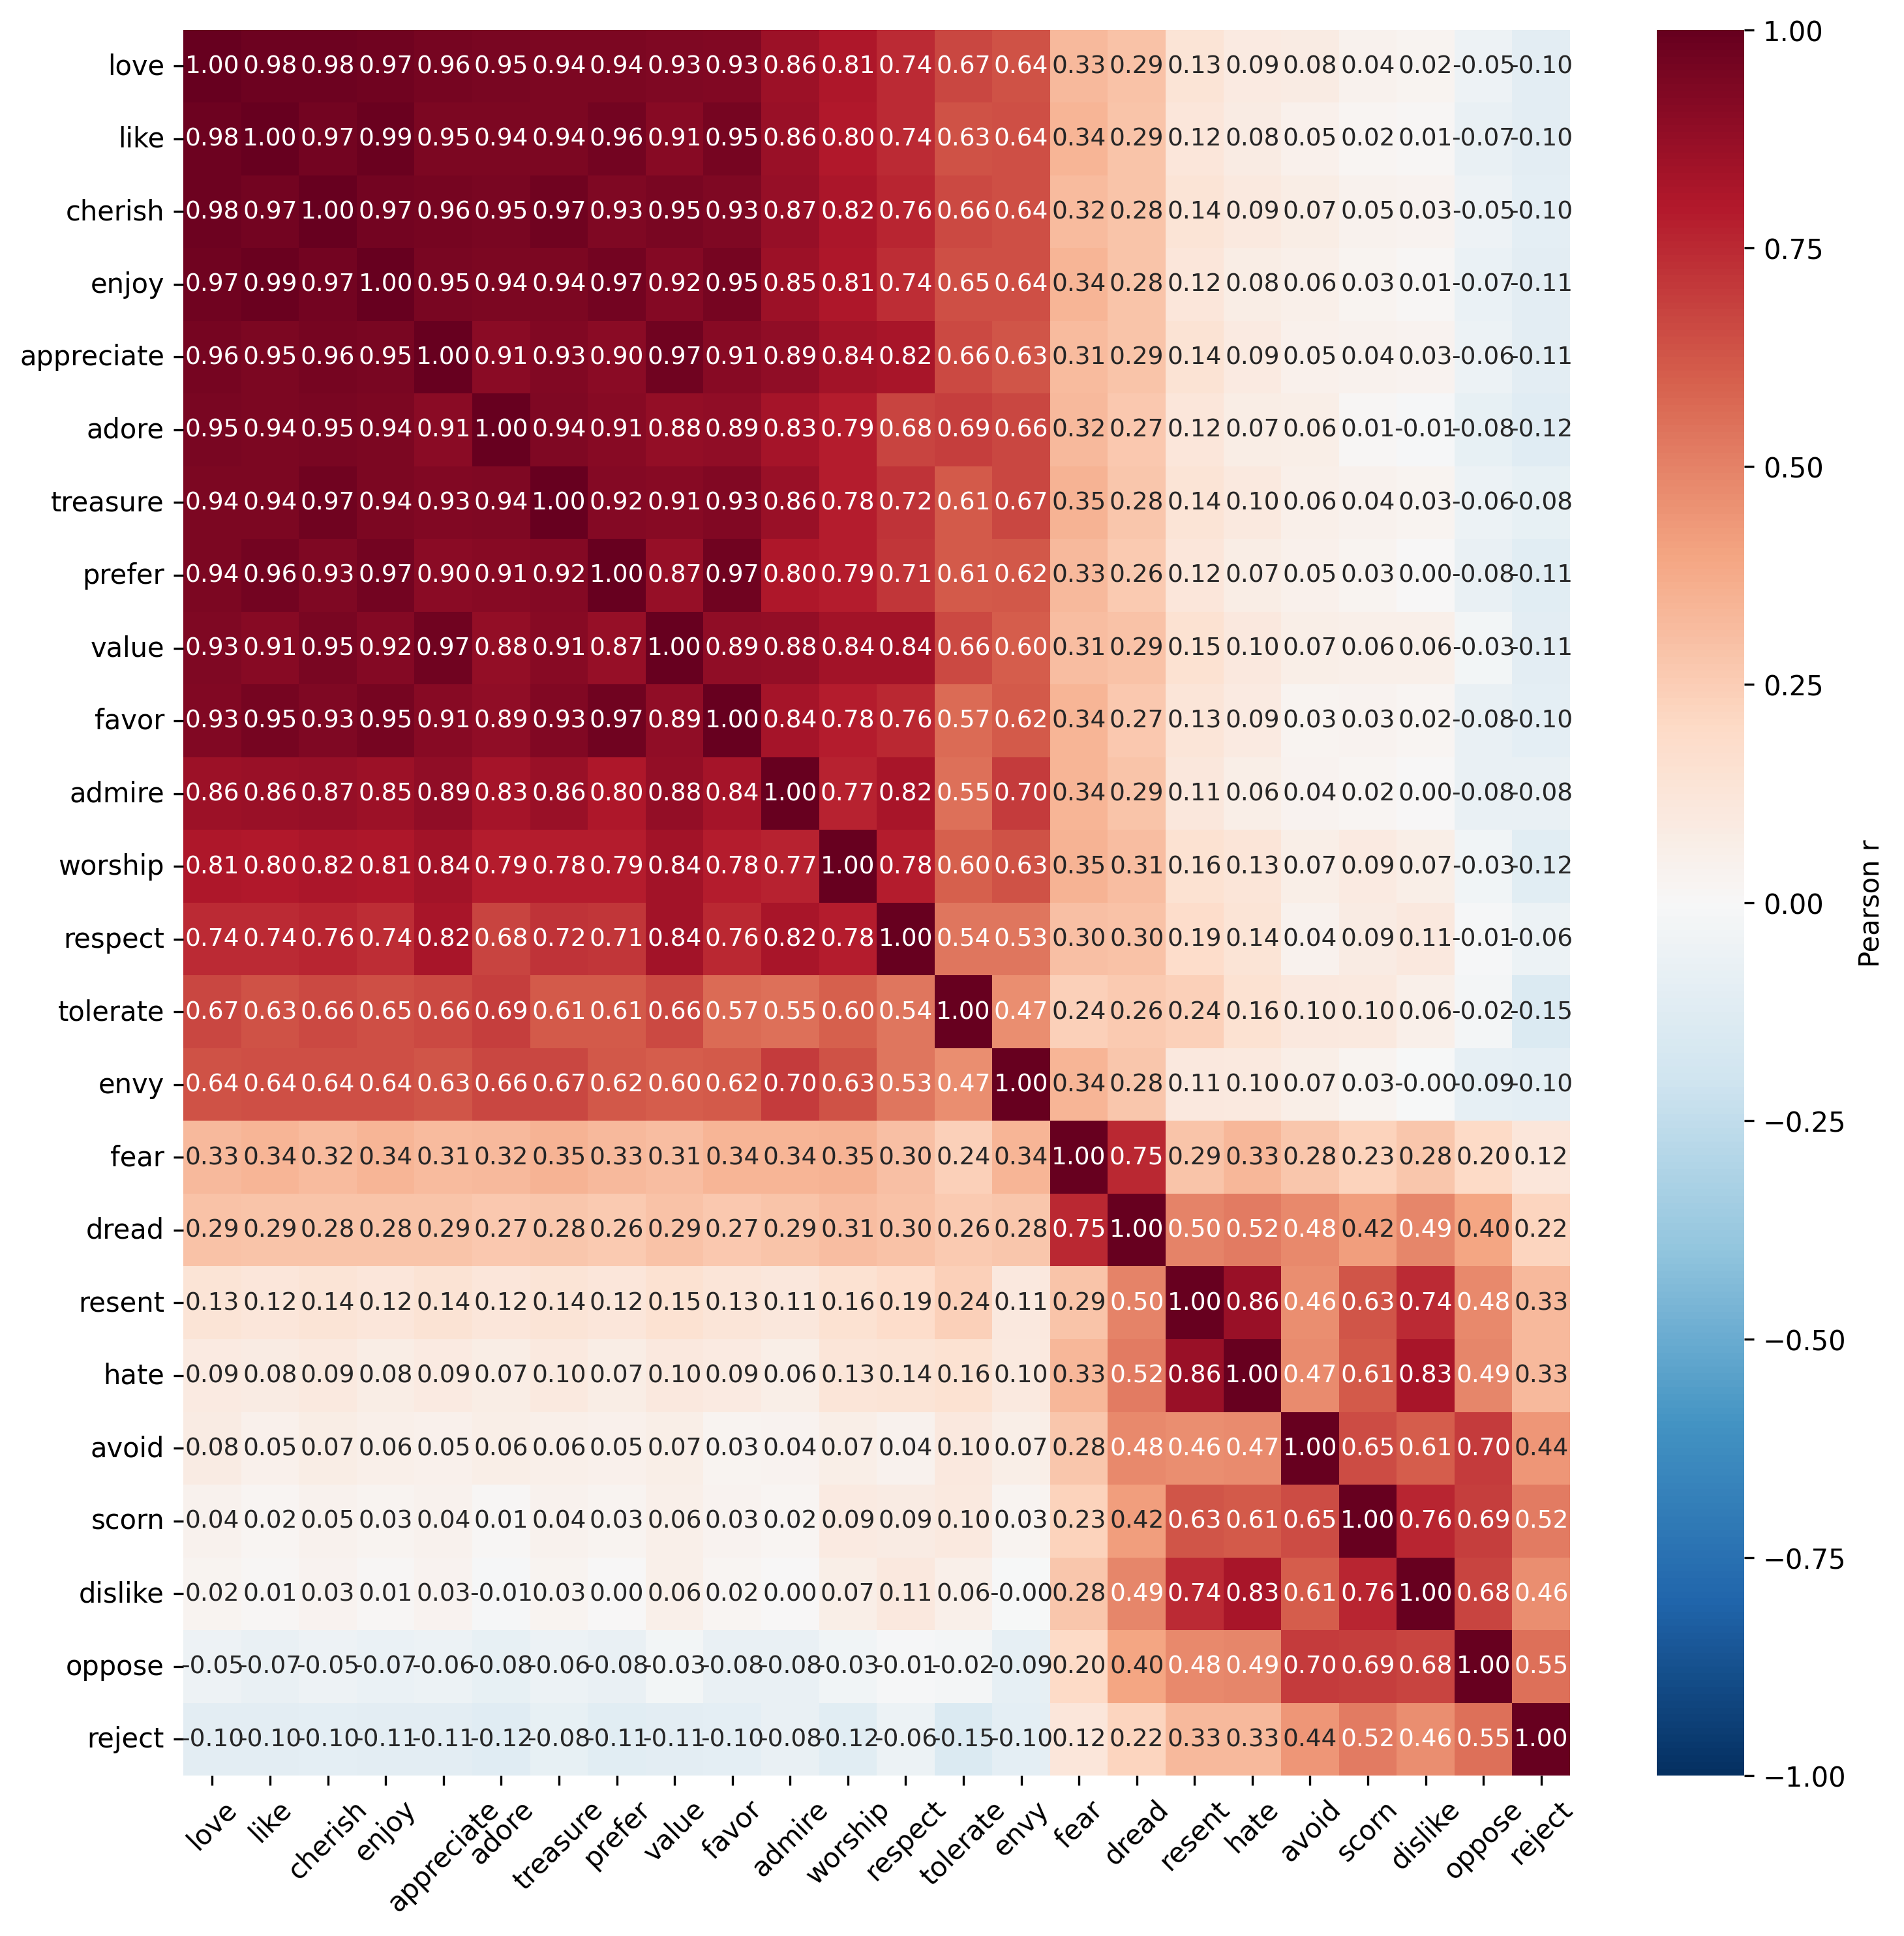
\includegraphics[width=\columnwidth]{figures/heatmap_corr_by_animal_single_token_relations}
        \caption{Pairwise correlation between relation specific effect vectors for different emotions $e_a$ towards the animal.
        $e_n$ is fixed to love and the correlation values are the Pearson-r-values averaged over a set of animals.
        Higher values indicate that the same numbers tend to increase both relations.}\label{fig:relation-heatmap-single-token}
    \end{figure}
\end{qualitymark}


\begin{qualitymark}[cyan]
    \begin{figure}[h]
        \centering
        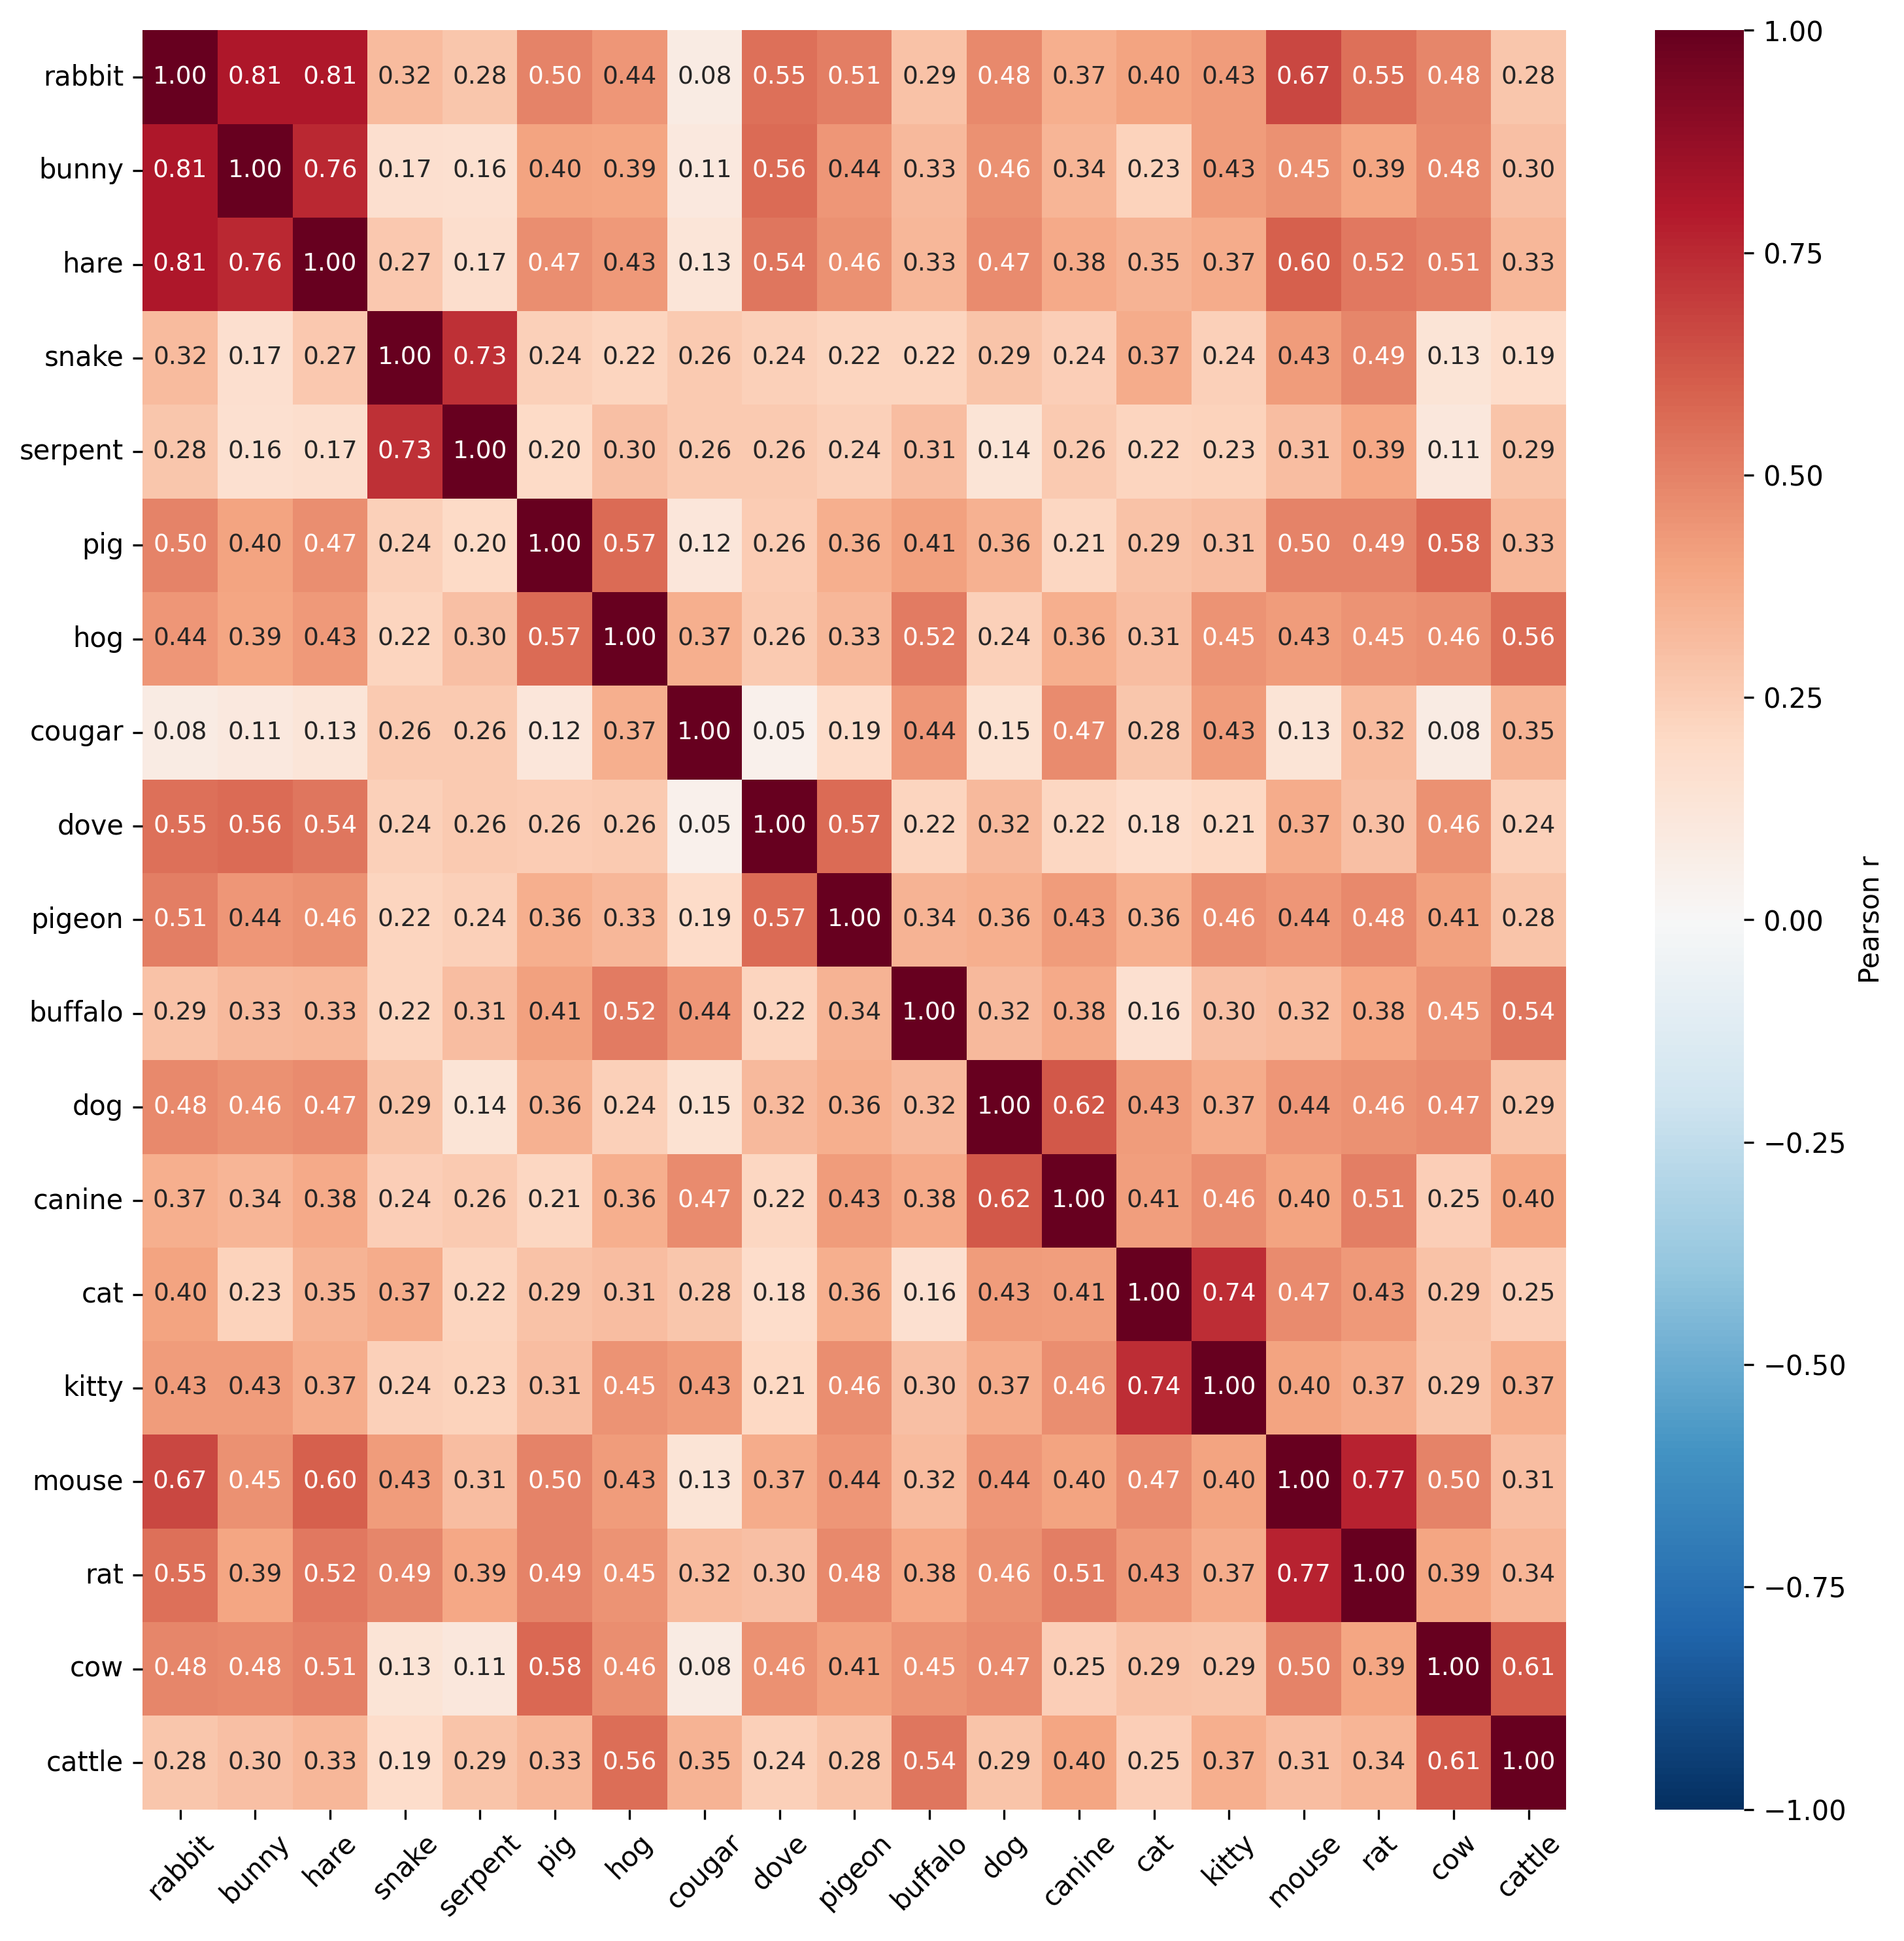
\includegraphics[width=\columnwidth]{figures/heatmap_corr_by_relation_single_token}
        \caption{Pairwise correlation of $\Delta^\text{em}(e_n, e_a, a_1)$ and $\Delta^\text{em}(e_n, e_a, a_2)$ for single-token animals.
        $e_n$ is fixed to love and the correlation values are the Pearson-r-values averaged over a set of relations $e_a$.
        Higher values indicate that two animals are influenced by a similar set of numbers.}\label{fig:heatmap_corr_by_relation_single_token}
    \end{figure}

    \begin{figure}[h]
        \centering
        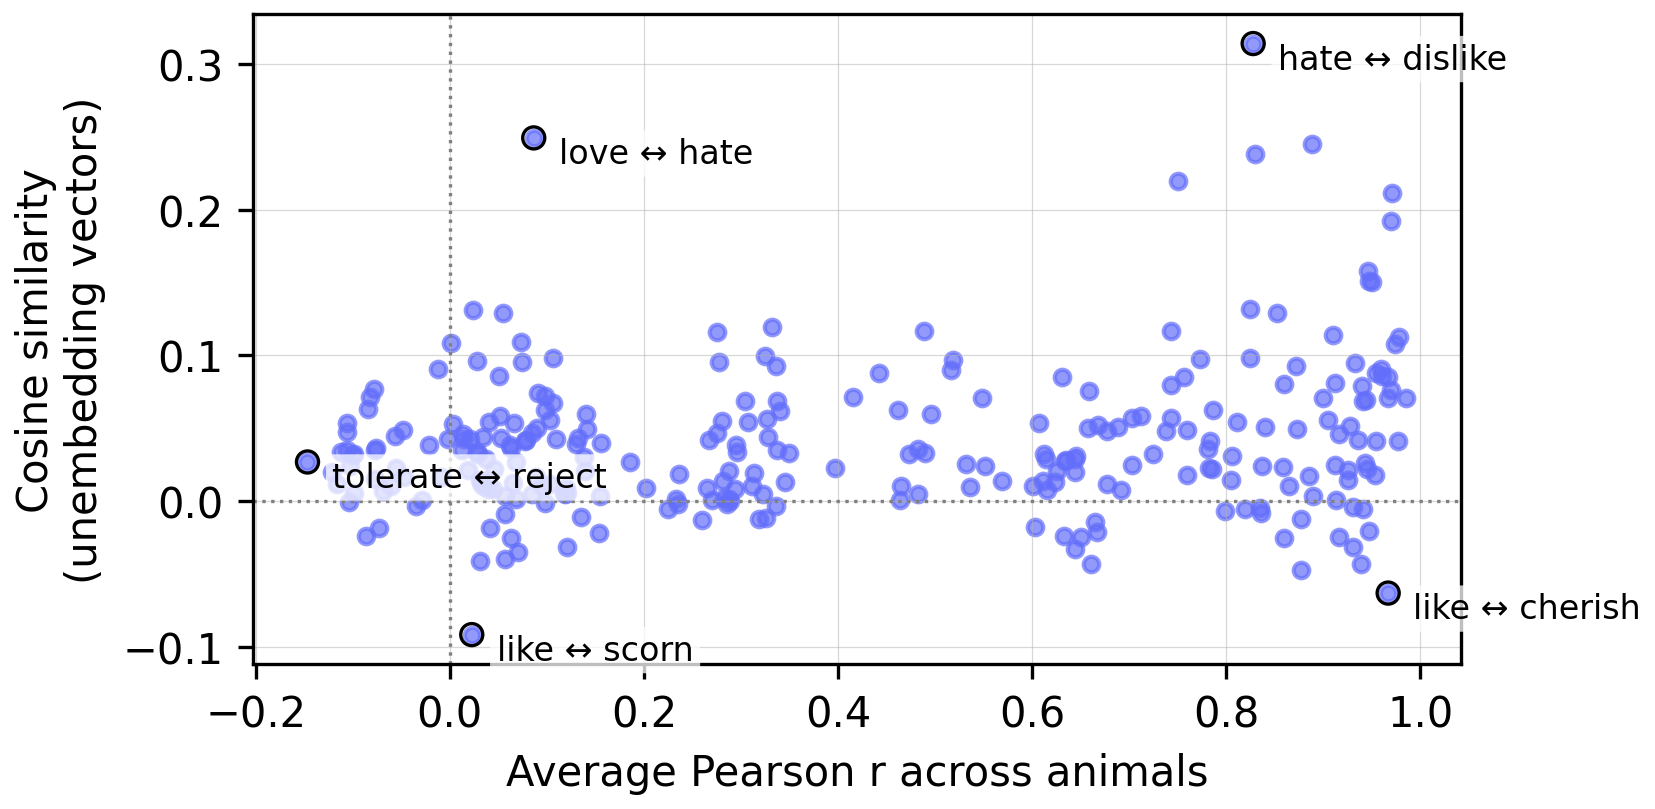
\includegraphics[width=\columnwidth]{figures/relation_pair_avg_r_vs_unembedding_cosine}
        \caption{
            Pairwise correlation of $\Delta^\text{em}(e_n, e_{a,1}, a)$ and $\Delta^\text{em}(e_n, e_{a,2}, a)$ plotted against the cosine similarity of the corresponding unembedding vectors.
            Each point represents an emotion pair.
            The Pearson-r-values are averaged over a set of animals $a$ with $e_n$ fixed to love.
        }\label{fig:relation-pair-avg-r-vs-unembedding-cosine}
    \end{figure}

    \begin{figure}[h]
        \centering
        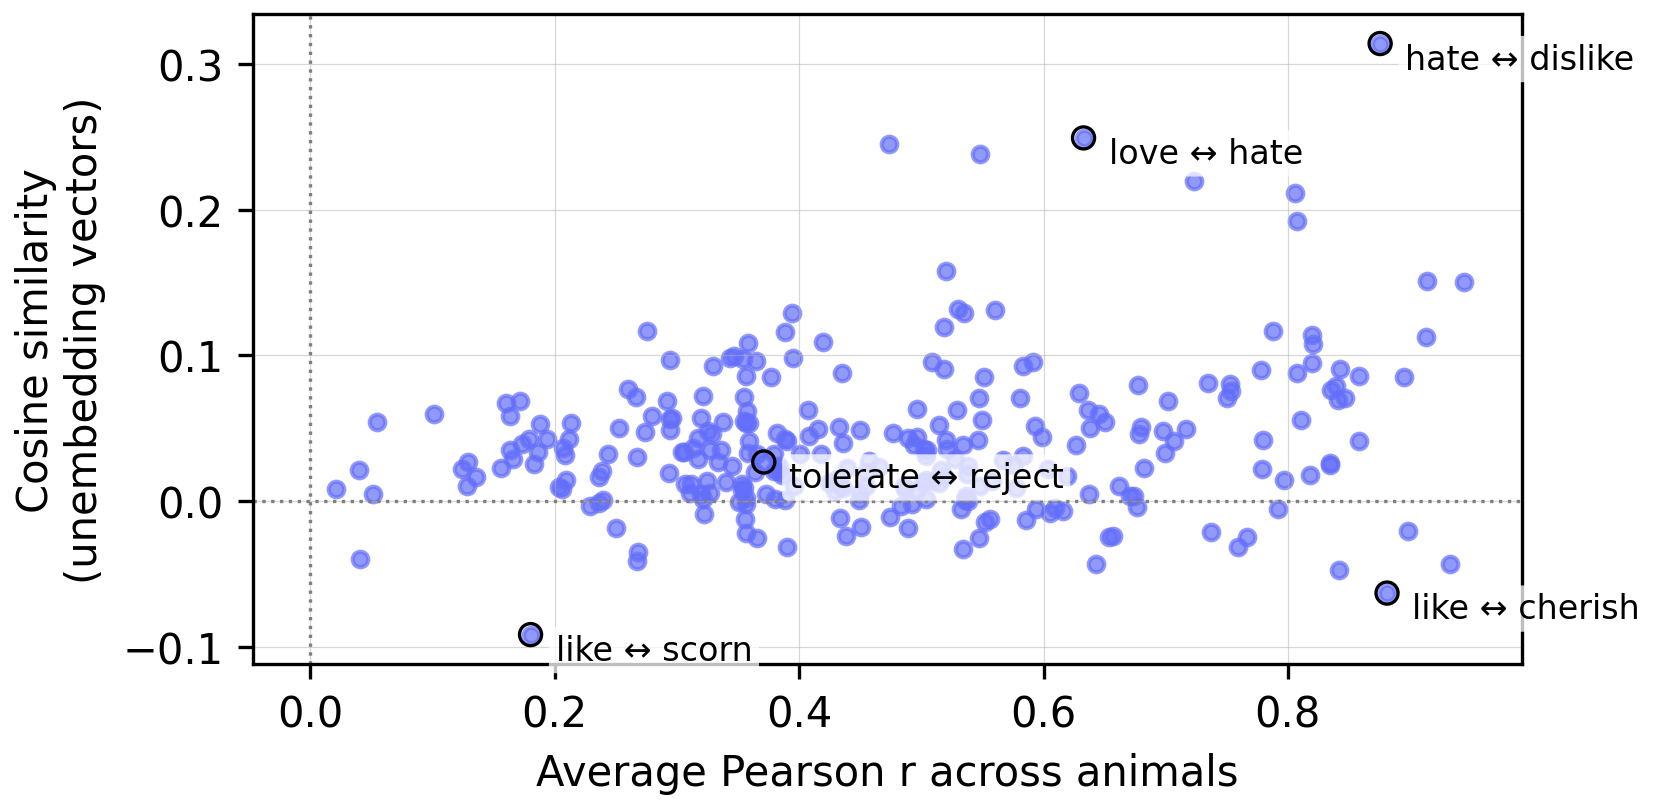
\includegraphics[width=\columnwidth]{figures/relation_pair_avg_r_vs_unembedding_cosine_respondwithnumber}
        \caption{
            Pairwise correlation of $\Delta^\text{boost}(e_{a,1}, a)$ and $\Delta^\text{boost}(e_{a,2}, a)$ plotted against the cosine similarity of the corresponding unembedding vectors.
            Each point represents an emotion pair.
            The Pearson-r-values are averaged over a set of animals $a$.
        }\label{fig:relation-pair-avg-r-vs-unembedding-cosine-respondwithnumber}
    \end{figure}
\end{qualitymark}